\subsection{Tan\-Ra\-Dec2Pix  Class Reference}
\label{class_tanradec2pix}\index{TanRaDec2Pix@{Tan\-Ra\-Dec2Pix}}
This one is the Tangent Plane (called gnomonic) projection (from celestial sphere to tangent plane). 


{\tt \#include $<$gtransfo.h$>$}

Inheritance diagram for Tan\-Ra\-Dec2Pix::\begin{figure}[H]
\begin{center}
\leavevmode
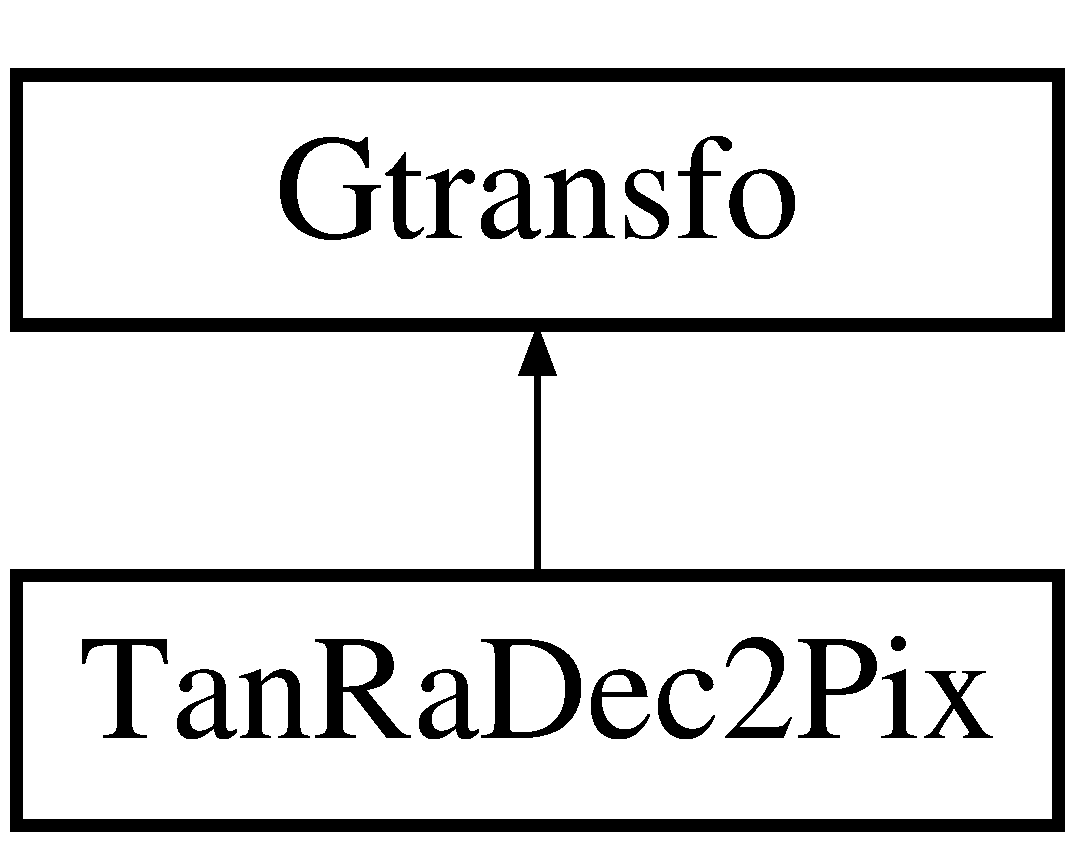
\includegraphics[height=2cm]{class_tanradec2pix}
\end{center}
\end{figure}
\subsubsection*{Public Methods}
\begin{CompactItemize}
\item 
\index{TanRaDec2Pix@{TanRaDec2Pix}!TanRaDec2Pix@{Tan\-Ra\-Dec2Pix}}\index{TanRaDec2Pix@{TanRaDec2Pix}!TanRaDec2Pix@{Tan\-Ra\-Dec2Pix}}
{\bf Tan\-Ra\-Dec2Pix} (const {\bf Gtransfo\-Lin} \&Tan2Pix, const {\bf Point} \&Tangent\-Point)\label{class_tanradec2pix_a0}

\begin{CompactList}\small\item\em assume degrees everywhere.\item\end{CompactList}\item 
\index{TanRaDec2Pix@{TanRaDec2Pix}!TanRaDec2Pix@{Tan\-Ra\-Dec2Pix}}\index{TanRaDec2Pix@{TanRaDec2Pix}!TanRaDec2Pix@{Tan\-Ra\-Dec2Pix}}
{\bf Tan\-Ra\-Dec2Pix} ()\label{class_tanradec2pix_a1}

\item 
\index{LinPart@{LinPart}!TanRaDec2Pix@{Tan\-Ra\-Dec2Pix}}\index{TanRaDec2Pix@{TanRaDec2Pix}!LinPart@{Lin\-Part}}
{\bf Gtransfo\-Lin} {\bf Lin\-Part} () const\label{class_tanradec2pix_a2}

\begin{CompactList}\small\item\em The Linear part (corresponding to CD's and CRPIX's).\item\end{CompactList}\item 
\index{TangentPoint@{TangentPoint}!TanRaDec2Pix@{Tan\-Ra\-Dec2Pix}}\index{TanRaDec2Pix@{TanRaDec2Pix}!TangentPoint@{Tangent\-Point}}
{\bf Point} {\bf Tangent\-Point} () const\label{class_tanradec2pix_a3}

\begin{CompactList}\small\item\em tangent point coordinates (in degrees).\item\end{CompactList}\item 
\index{apply@{apply}!TanRaDec2Pix@{Tan\-Ra\-Dec2Pix}}\index{TanRaDec2Pix@{TanRaDec2Pix}!apply@{apply}}
void {\bf apply} (const double Xin, const double Yin, double \&Yout, double \&Yout) const\label{class_tanradec2pix_a4}

\item 
\index{invert@{invert}!TanRaDec2Pix@{Tan\-Ra\-Dec2Pix}}\index{TanRaDec2Pix@{TanRaDec2Pix}!invert@{invert}}
{\bf Tan\-Pix2Ra\-Dec} {\bf invert} () const\label{class_tanradec2pix_a5}

\begin{CompactList}\small\item\em exact typed inverse:.\item\end{CompactList}\item 
\index{RoughInverse@{RoughInverse}!TanRaDec2Pix@{Tan\-Ra\-Dec2Pix}}\index{TanRaDec2Pix@{TanRaDec2Pix}!RoughInverse@{Rough\-Inverse}}
{\bf Gtransfo}$\ast$ {\bf Rough\-Inverse} (const {\bf Frame} \&Region) const\label{class_tanradec2pix_a6}

\begin{CompactList}\small\item\em Overload the \char`\"{}generic routine\char`\"{} (available for all {\bf Gtransfo} {\rm (p.\,\pageref{class_gtransfo})} types.\item\end{CompactList}\item 
\index{InverseTransfo@{InverseTransfo}!TanRaDec2Pix@{Tan\-Ra\-Dec2Pix}}\index{TanRaDec2Pix@{TanRaDec2Pix}!InverseTransfo@{Inverse\-Transfo}}
{\bf Gtransfo}$\ast$ {\bf Inverse\-Transfo} (const double Precision, const {\bf Frame} \&Region) const\label{class_tanradec2pix_a7}

\begin{CompactList}\small\item\em Inverse transfo: returns a {\bf Tan\-Pix2Ra\-Dec} {\rm (p.\,\pageref{class_tanpix2radec})}.\item\end{CompactList}\item 
\index{dump@{dump}!TanRaDec2Pix@{Tan\-Ra\-Dec2Pix}}\index{TanRaDec2Pix@{TanRaDec2Pix}!dump@{dump}}
void {\bf dump} (ostream \&stream) const\label{class_tanradec2pix_a8}

\begin{CompactList}\small\item\em dumps the transfo coefficients to stream.\item\end{CompactList}\item 
\index{Clone@{Clone}!TanRaDec2Pix@{Tan\-Ra\-Dec2Pix}}\index{TanRaDec2Pix@{TanRaDec2Pix}!Clone@{Clone}}
{\bf Gtransfo}$\ast$ {\bf Clone} () const\label{class_tanradec2pix_a9}

\begin{CompactList}\small\item\em returns a copy (allocated by new) of the transformation.\item\end{CompactList}\item 
double {\bf fit} (const Star\-Match\-List \&List, const {\bf Gtransfo} $\ast$Prior\-Transfo=NULL, const {\bf Gtransfo} $\ast$Posterior\-Transfo=NULL)
\begin{CompactList}\small\item\em fits a transfo to a list of star pairs (p1,p2).\item\end{CompactList}\end{CompactItemize}


\subsubsection{Detailed Description}
This one is the Tangent Plane (called gnomonic) projection (from celestial sphere to tangent plane).

this transfo does not implement corrections, since  they are defined the other way around (from pixels to sky),  and not invertible analytically. The inversion of tangent point WCS ({\bf Tan\-Pix2Ra\-Dec} {\rm (p.\,\pageref{class_tanpix2radec})}) is obtained via {\bf Inverse\-Transfo}() {\rm (p.\,\pageref{class_tanradec2pix_a7})}. 



\subsubsection{Member Function Documentation}
\index{TanRaDec2Pix@{Tan\-Ra\-Dec2Pix}!fit@{fit}}
\index{fit@{fit}!TanRaDec2Pix@{Tan\-Ra\-Dec2Pix}}
\paragraph{\setlength{\rightskip}{0pt plus 5cm}double Tan\-Ra\-Dec2Pix::fit (const Star\-Match\-List \& {\em List}, const {\bf Gtransfo} $\ast$ {\em Prior\-Transfo} = NULL, const {\bf Gtransfo} $\ast$ {\em Posterior\-Transfo} = NULL)\hspace{0.3cm}{\tt  [virtual]}}\hfill\label{class_tanradec2pix_a10}


fits a transfo to a list of star pairs (p1,p2).

After the fit this(Prior\-Transfo(p1)) yields approximately Posterior\-Transfo(p2). The returned value is the chi2. 

Reimplemented from {\bf Gtransfo} {\rm (p.\,\pageref{class_gtransfo_a4})}.

The documentation for this class was generated from the following file:\begin{CompactItemize}
\item 
{\bf gtransfo.h}\end{CompactItemize}
